% Keep diagram labels single-spaced, independently of the thesis body.
\begingroup
\linespread{1}\selectfont
\begin{tikzpicture}[
  imgnode/.style={inner sep=0pt, draw=black!35, line width=1.0pt},
  boxnode/.style={draw=black!70, rounded corners=2pt, minimum height=0.8cm, minimum width=1.2cm, align=center, font=\small, fill=black!3, inner sep=4pt},
  arr/.style={-{Latex[length=2.2mm,width=1.6mm]}, very thick, black!65},
  titletext/.style={font=\bfseries},
  captiontext/.style={font=\small\itshape, align=center, text width=7.2cm},
]

% ---------- left: passive perception ----------
% same crop as the active side's "what it sees" -- the passive model is simply
% handed, for free, the exact view the active agent had to act to obtain.
\node[imgnode] (fullscene) {
\includegraphics[width=2.4cm]{figures/img/main/three/renders/passive_active_camera.png}};
\node[boxnode, right=0.55cm of fullscene] (model1) {Model};
\node[right=0.55cm of model1, font=\bfseries] (out1) {\textquotedblleft tree\textquotedblright};

\draw[arr] (fullscene) -- (model1);
\draw[arr] (model1) -- (out1);

\node[fit=(fullscene)(model1)(out1), inner sep=0pt] (leftgroup) {};
\node[captiontext, below=0.45cm of leftgroup] (leftcap2) {(single feed-forward pass)};

% ---------- right: active embodied vision ----------
% anchored off "out1" (the true rightmost element of the left group), not
% "fullscene" -- anchoring off fullscene alone let this group overlap model1/out1.
\node[imgnode, right=1.2cm of out1] (scene3p) {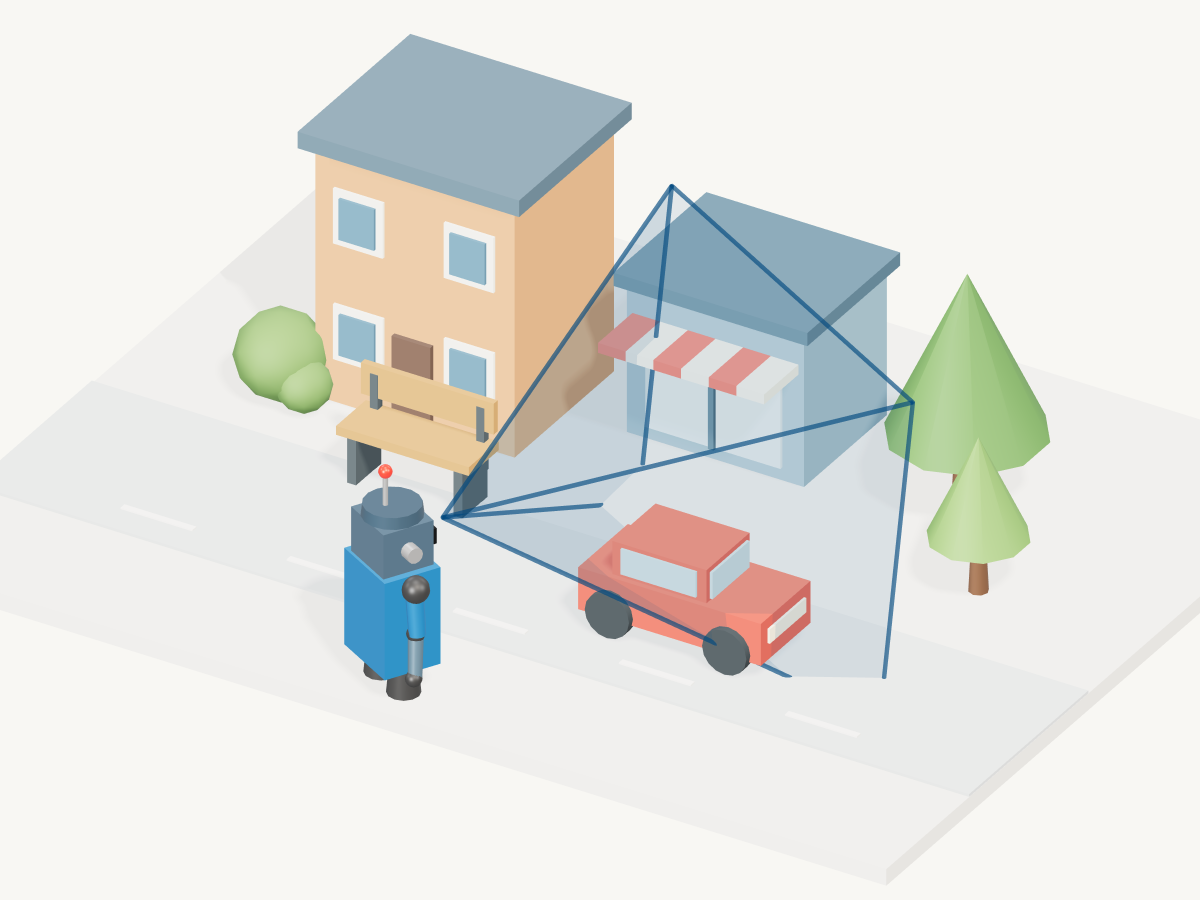
\includegraphics[width=3.1cm]{figures/img/main/three/renders/passive_active_overview.png}};
\node[imgnode, right=0.55cm of scene3p, label=above:{\small camera view}] (scene1p) {
\includegraphics[width=1.55cm]{figures/img/main/three/renders/passive_active_camera.png}};
\node[boxnode, right=0.55cm of scene1p] (model2) {Model};

\draw[arr] (scene3p) -- (scene1p);
\draw[arr] (scene1p) -- (model2);

% the action closes the loop: model -> scene (it moves/looks, producing the
% next observation). The action text sits just below this arrow, as its caption.
% loopbottom is anchored below scene3p (not model2) so the final vertical run
% into scene3p.south is always comfortably longer than the corner-rounding
% radius -- too short a run there left the arrowhead angled instead of pointing
% straight up into the image.
\coordinate (loopbottom) at ($(scene3p.south)+(0,-0.5)$);
\coordinate (loopcorner) at (model2.south |- loopbottom); % x of model2.south, y of loopbottom
\draw[arr, rounded corners=7pt] (model2.south) -- (loopcorner) -- (loopbottom) -- (scene3p.south);

\path (scene3p.south) -- (model2.south) coordinate[midway] (loopmid);
\node[align=center, font=\bfseries\small, anchor=north] (actA) at ($(loopmid)+(-0,-1.0)$) {move forward and look to the right};

\node[fit=(scene3p)(scene1p)(model2)(actA), inner sep=0pt] (rightgroup) {};
\node[titletext, above=1cm of rightgroup] (righttitle) {Active embodied vision};
\node[captiontext, text width=7.2cm] (rightcap) at ($(righttitle.center)+(0,-0.57)$) {the agent acts to decide what to observe next};
% Share text baselines across panels independently of their content heights.
\node[titletext, anchor=base] (lefttitle) at (leftgroup.center |- righttitle.base) {Passive perception};
\node[captiontext, anchor=base] (leftcap) at (leftgroup.center |- rightcap.base) {complete visual information provided};
\node[captiontext, below=0.15cm of rightgroup] (rightcap2) {(observe $\to$ move $\to$ repeat)};

% Match the divider to the visible panel content; avoid caption padding.
\coordinate (divider) at ($(leftgroup.east)!0.5!(scene3p.west)$);
\draw[black!45, line width=0.4pt]
  (divider |- righttitle.north) -- (divider |- rightcap2.south);

\end{tikzpicture}
\endgroup
